\speciestitle{Nitrous Oxide}{N\cs2O}{N2O}{%
\item[Useful range:] 68\,--\,0.46\,hPa
\item[Contact:] Alyn Lambert, \email{Alyn.Lambert@jpl.nasa.gov}}

\subsection{Introduction}

\subsubsection{Redefinition of the N\cs2O standard product for \thisv
  to use band 3 (190-GHz) signals}

The standard product for \thisv N\cs2O is taken from the 190-GHz
(``Core+R2'') retrieval (\texttt{N2O-190}) instead of the 640-GHz (``Core+R4B'')
retrieval (\texttt{N2O-640}) as used in previous versions.

Aging of the MLS ``band~12'' (640-GHz) signals was revealed by analysis
of housekeeping data during June-August 2013 which showed declining
output in counts, increasing radiance noise (variance) and also
increasing correlation between the band 12 radiance channels. As the
640\,GHz N\cs2O product began to show further deterioration in quality a
decision was made to turn off band 12 on August 6, 2013. Prior to that,
the level-2 processing stream for the N\cs2O standard product in v3.x
was switched to output the ``band~3'' (190-GHz, \texttt{N2O-190}) retrieval
on 7~June 2013 and later data for \texttt{N2O-640} are not recommended
for scientific use.

The 190-GHz N\cs2O data show slightly worse precision and resolution
compared to the 640-GHz retrievals. Data from \texttt{N2O-190} and
\texttt{N2O-640} have been compared from launch until the end of band 12
operations. There is a persistent high bias in \texttt{N2O-190} of
$>30\%$ at 100 hPa (although some seasonal variations are evident) and
we recommend that at this particular pressure level \texttt{N2O-190}
only be used in consultation with the MLS science team.  A smaller bias
of 5--10\% at 68\,hPa in \texttt{N2O-190} is seen compared to
\texttt{N2O-640}. From 46 to 3.2\,hPa the biases are less than 5\% (see
Figure~\ref{fig:N2O190640Comparison}).

\begin{figure}
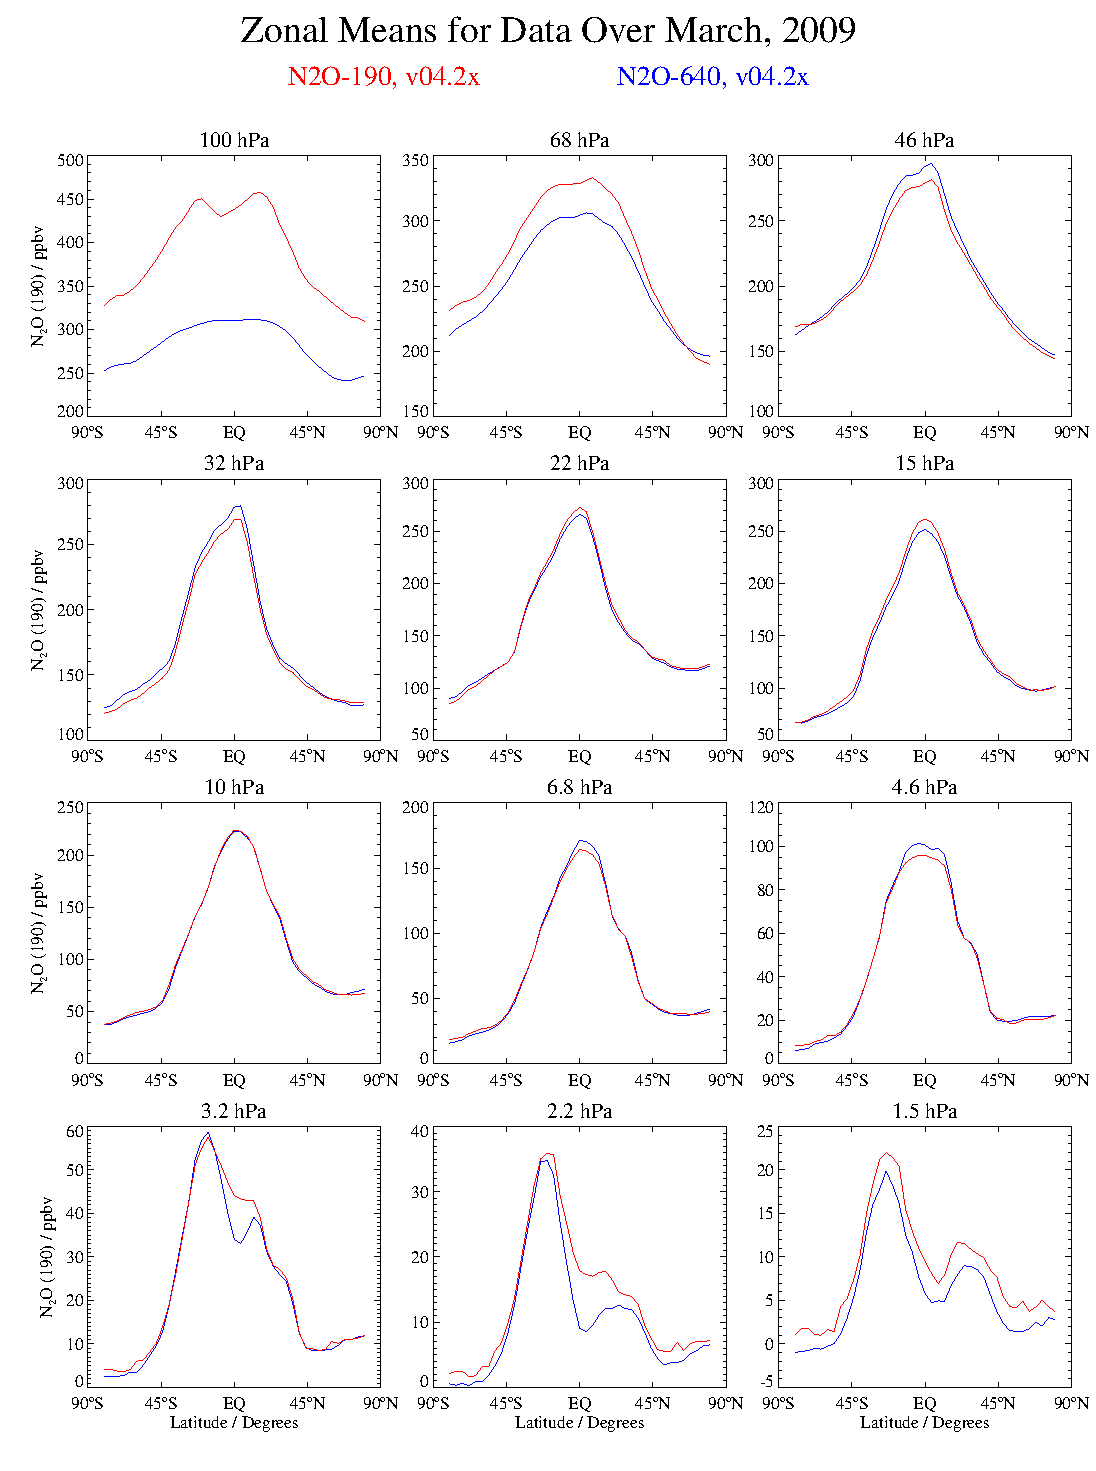
\includegraphics[width=\linewidth]{figures/InspectZM_2009m03_N2O-190-v04-2x_N2O-640-v04-2x_userHeightRange}
\caption{MLS \thisv \texttt{N2O-190} and \texttt{N2O-640} comparison for
  March 2009}
\label{fig:N2O190640Comparison}
\end{figure}

Other significant differences between the \thisv \texttt{N2O-190} and
\texttt{N2O-640} data such as the resolution, precision, recommended pressure levels, 
quality and convergence criteria are noted below.

The secondary \thisv N\cs2O 640-GHz product is available for the period
from launch until June 6, 2013 and stored in the \texttt{L2GP-DGG} files
in the \texttt{N2O-640} swath.  Details of the retrieval method and
validation results are presented in \citep{LambertEtal:2007}.

\subsection{Resolution}

\onestandardavk{N2O-190}{190\,GHz N\cs2O}

\onestandardavk{N2O-640}{640\,GHz N\cs2O}

The spatial resolution reported by the averaging kernel matrices is
shown in Figures~\ref{fig:AvkN2O-190} for the 190\,GHz measurements
and~\ref{fig:AvkN2O-640} for the 640\,GHz measurements (available in the
\texttt{L2GP-DGG} files for data prior to June~6, 2013).  For
\texttt{N2O-190}, the vertical resolution is 4\,--\,8\,km and the
horizontal along-track resolution is 300\,--\,600\,km.  For
\texttt{N2O-640}, the vertical resolution is 4\,--\,6\,km and the
horizontal along-track resolution is 300\,--\,600\,km over most of the
useful range of the retrievals.

The horizontal cross-track resolution is set by the 7\,km width of the
MLS 190-GHz field-of-view for all pressures. Note that the higher
frequency MLS 640-GHz measurements have a narrower 3\,km field-of-view.
The longitudinal separation of the MLS measurements is
10\degsym--\,20\degsym\ over middle and lower latitudes, with much finer
sampling in polar regions.

\subsection{Precision}

Precision as defined here is the $1\sigma$ uncertainty in the retrieved
value calculated by the Level~2 algorithms and has been validated
against the scatter about the mean of coincident ascending/descending
MLS profile differences.  The estimated precision on a single retrieved
profile given in Tables~\ref{tab:N2OSummary} and~\ref{tab:N2O640Summary}
varies with height from \texttildelow15\,--\,20\,ppbv for \texttt{N2O-190} and
\texttildelow12\,--\,25\,ppbv for \texttt{N2O-640}.

The N\cs2O values at the 147\,hPa pressure level have a large a priori
influence and practically all precisions are flagged negative at this
level.

\subsection{Accuracy}

The accuracy values given in Table~\ref{tab:N2O640Summary} were obtained
for both v4 N\cs2O products using the same detailed analyses presented
for MLS \texttt{N2O-640} v2.2 data in \citet{LambertEtal:2007} to quantify
the systematic uncertainties associated with the MLS instrument
calibration, spectroscopic uncertainty and approximations in the
retrieval formulation and implementation.

\subsection{Data screening}
\label{sec:N2OScreening}
\begin{description}
\item[Pressure range (\texttt{N2O-190}):] \screeningrule{68\,--\,0.46\,hPa}
\item[Pressure range (\texttt{N2O-640}):] \screeningrule{100\,--\,0.46\,hPa}
\standardrangestatement\ In the upper stratosphere and lower
  mesosphere \thisv N\cs2O requires significant averaging for useful
  signals, but see the note under ``Artifacts'' for issues at pressures below
  0.1\,hPa.

\standardprecisionrule
\evenstatusrule

\item[Quality (\texttt{N2O-190}):] \qualityrule{1.0} Note that this is a
  change from the threshold originally suggested for \thisv.  See the
  discussion of this topic below.

\item[Convergence (\texttt{N2O-190}):] \convergencerule{2.0}
  A fraction of the \texttt{N2O-190} data (typically less than 0.5\%) at this level
  will be discarded via this screening.

\item[Quality (\texttt{N2O-640}):] \qualityrule{1.4}
  A small fraction of \texttt{N2O-640} profiles (typically less than 0.5\%) will
  be discarded via this screening.

\item[Convergence (\texttt{N2O-640}):] \convergencerule{1.01}
  A fraction of the \texttt{N2O-640} data (typically less than 0.5\%) at this level
  will be discarded via this screening.

\item[Clouds:] \screeningrule{Clouds have little impact on the N\cs2O products at the recommended pressure levels. 
Ignore status bit 16 (high cloud) or bit 32 (low cloud) indicating the presence of clouds. See
artifacts for more details.}

\end{description}

\subsubsection{Updated \texttt{Quality} screening recommendation}
A byproduct of the aging in MLS that gives rise to the drift in the
water vapor product (see section~\ref{sec:H2ODrift}) and 190-GHz N\cs2O
(see below) is that the \texttt{Quality} metric for the 190-GHz N\cs2O
product exhibits a decreasing trend (most notable in the years following
\texttildelow2009).  This decrease is not correlated with any actual
decline in the accuracy of the MLS N\cs2O product, which appears largely
unchanged (drift issues aside).  However, application of the previously
recommended 1.3 \texttt{Quality} threshold leads to rejection of an
unreasonably large fraction of the N\cs2O profiles in the more recent
years of the Aura mission, particularly during southern winter.  The
revised 1.0 \texttt{Quality} threshold restores these profiles without
erroneously identifying any obviously poor profiles as acceptable.

\subsection{Artifacts}
\label{sec:N2ODrift}

In addition to the large bias of the 190-GHz N\cs2O at 100\,hPa (not
removed by screening), there are occasional outliers at the highest
presure levels in \texttt{N2O-190} and \texttt{N2O-640} products. 
Very thick clouds in the tropics produce a low rate of artifacts in the \thisv N\cs2O
products since improvements in the handling of radiances affected by
clouds have reduced the frequency of outliers compared to previous
versions. The cloud bits of the \texttt{Status} field are too blunt a
tool to identify these rare cases, needlessly discarding reasonable data.
Screening using the convergence
and quality fields (see above) is recommended to remove the majority of
these data points. 

The retrieval restricts N\cs2O values to be greater than
$-40\,\text{ppbv}$ (approximately three times the retrieval noise level
in the recommended pressure range) in order to prevent problems in the
minimization search process.  The low bound is applied at all levels,
but it is only evident in the data for pressures less than 0.1\,hPa,
where the vertical smoothing is relaxed and the retrieval noise becomes
comparable to the magnitude of the low bound value.  Accordingly,
statistical averaging of the data (zonal means or longer time periods)
cannot be applied successfully for pressures at and less than 0.1\,hPa
as the $-40\,\text{ppbv}$ hard limit introduces a positive bias in any
average.

A long-term trend of about $-0.5\%$ per year has been observed in the
MLS \texttt{N2O-190} data product, through analysis of the mean values
in the equatorial lower stratosphere in the years following 2009.  Since
the long term secular increase in tropospheric N\cs2O observed by
ground-based instruments is about $+0.25\%/\text{year}$, the anomalous
MLS \texttt{N2O-190} drift giving rise to the observed \texttt{N2O-190}
trend is probably around $-0.75\%/\text{year}$. The cause of this small
but statistically significant drift is under investigation.

\subsection{Review of comparisons between MLS N\cs2O  versions and other datasets}

Average values for \thisv 190-GHz N\cs2O are up to 10\% smaller than in v2.2 for the
100 and 68\,hPa pressure levels, and within a few percent for pressures greater than 46\,hPa 
(see Figure~\ref{fig:N2O190Comparison}). Differences between \thisv 190-GHz N\cs2O and
v3.3 are less than a few percent at all levels.

\begin{figure}
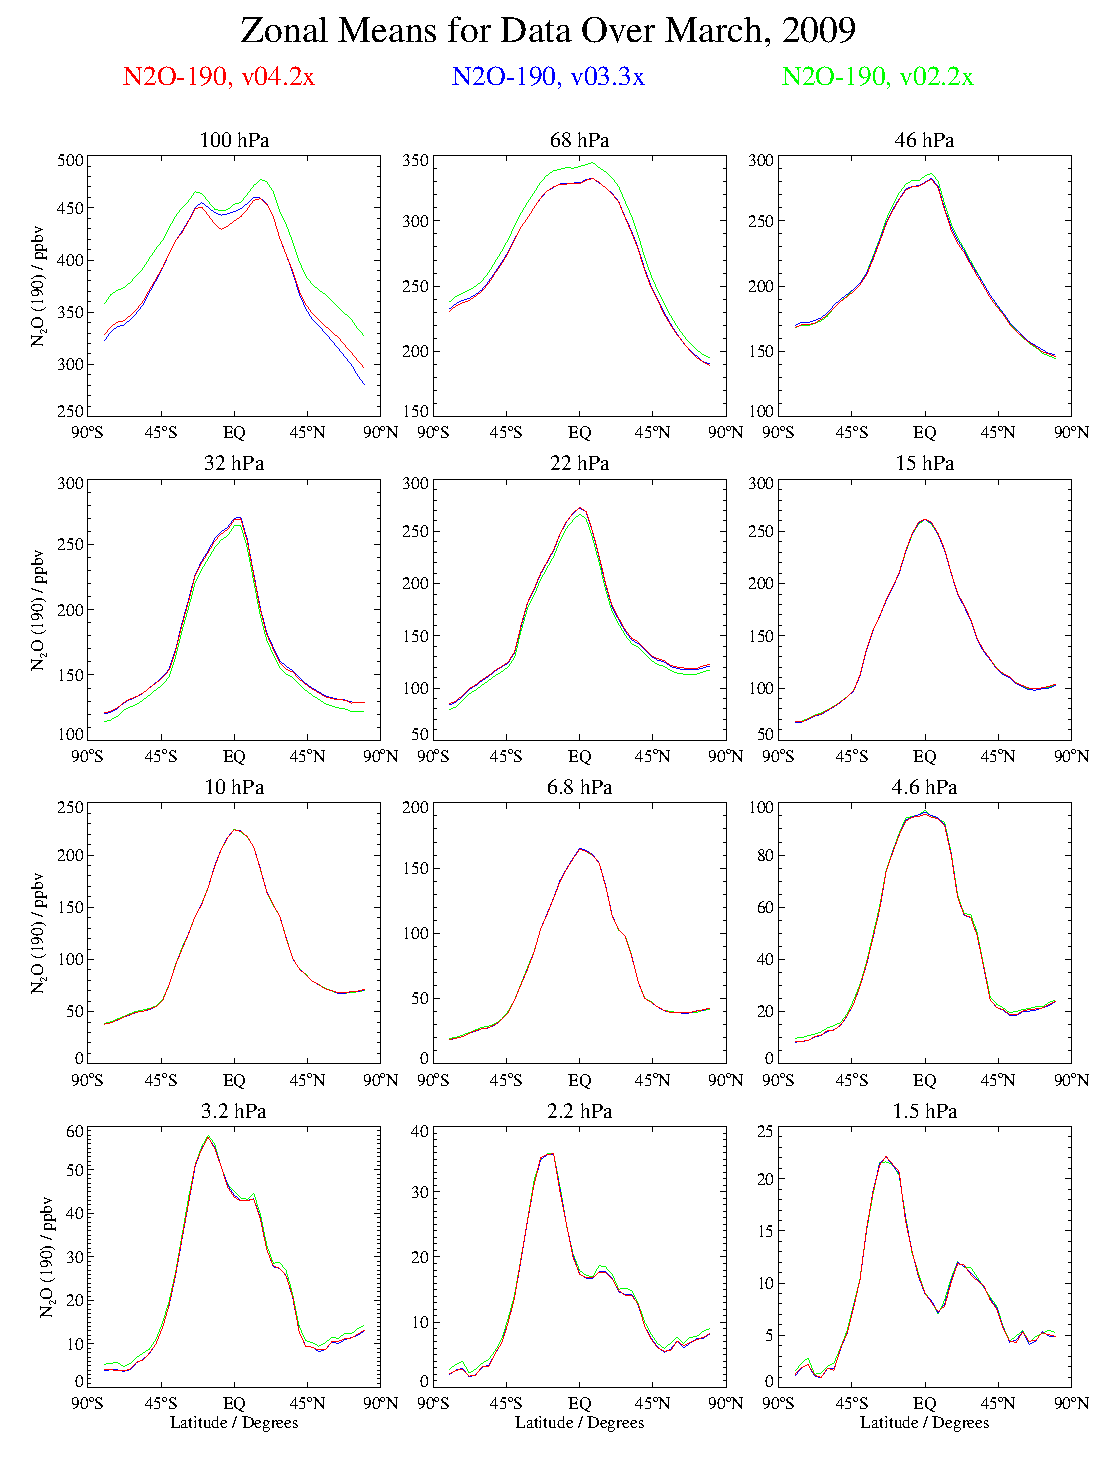
\includegraphics[width=\linewidth]{figures/InspectZM_2009m03_N2O-190-v04-2x_N2O-190-v03-3x_N2O-190-v02-2x_userHeightRange}
 \caption{MLS v4.2 190-GHz N\cs2O compared to v2.2 and v3.3 for March 2009}
\label{fig:N2O190Comparison}
\end{figure}

Average values for \thisv 640-GHz N\cs2O are 20\% larger than in v2.2
for the 100\,hPa pressure level, up to 10\% smaller at the
46\,--\,32\,hPa levels, and within 5\% for pressures greater than
22\,hPa (see Figure~\ref{fig:N2O640Comparison}). Differences between
\thisv 640-GHz N\cs2O and v3.3 are less than a few percent at all
levels. Unlike the \texttt{N2O-190} product, the \texttt{N2O-640}
product is recommended for scientific use at 100\,hPa.

Apart from the differences noted above, the MLS \thisv 640 GHz N\cs2O is
similar to the MLS v2.2 product described and validated in
\citet{LambertEtal:2007}.  Comparisons of v2.2 640 GHz N\cs2O with
coincident measuremements by ACE-FTS, Odin/SMR, and Envisat/MIPAS and
balloon borne observations are shown in \citet{LambertEtal:2007}.  A
revised validation paper for N\cs2O is not planned in the near future
and users are encouraged to read \citet{LambertEtal:2007} for more
information.

\begin{figure}
  \includegraphics[width=\linewidth]{figures/InspectZM_2009m03_N2O-640-v04-2x_N2O-640-v03-3x_N2O-640-v02-2x_userHeightRange}
 \caption{MLS v4.2 640 GHz N\cs2O compared to v2.2 and v3.3 for March 2009}
\label{fig:N2O640Comparison}
\end{figure}

\subsection{Desired improvements for future data version(s)}

Retrievals of N\cs2O to pressures greater than 100\,hPa \emph{may} be
possible in later versions from the 190-GHz observations.

\begin{table}[b]
  \caption{Summary of MLS \thisv N\cs2O (\texttt{N2O-190}) product.}\vspace{0.5ex}
\label{tab:N2OSummary}
\begin{minipage}{\linewidth}
\centering\begin{tabular}{ccccccl}
\toprule
\parbox[m]{15mm}{\centering\textbf{Region}} &
\parbox[m]{24mm}{\centering\textbf{Resolution\\ Vert. $\times$ Horiz.}} &
\multicolumn{2}{c}{\parbox[m]{18mm}{\centering\textbf{Precision\footnote{Precision on individual profiles}}}} &
\multicolumn{2}{c}{\parbox[m]{15mm}{\centering\textbf{Accuracy}}} &
\textbf{Comments} \\
\textbf{hPa} & \textbf{km} &  \textbf{ppbv} & \textbf{\%} & \textbf{ppbv} & \textbf{\%} & \\
\midrule
$\leq$0.33   & ---                 & ---   & ---       & --- & --- & Unsuitable for scientific use \\   
0.46         &  11.0 $\times$  655 &   15  & $>$100 &  2  & $>$100 & \\ 
0.68         &   9.7 $\times$  540 &   17  & $>$100 &  2  & 89 & \\ 
1.0          &   8.6 $\times$  440 &   18  & $>$100 &  2  & 50 & \\ 
2.2          &   7.3 $\times$  340 &   19  &   64   &  4  & 36 & \\ 
4.6          &   6.5 $\times$  285 &   17  &   23   &  5  & 11 & \\ 
10           &   6.0 $\times$  265 &   16  &   12   &  7  &  7 & \\ 
22           &   5.6 $\times$  305 &   15  &    9   & 10  &  6 & \\ 
46           &   4.9 $\times$  385 &   14  &    7   & 30  & 10 & \\ 
68           &   5.4 $\times$  420 &   16  &    6   & 55  & 22 & \\
100          &   3.8 $\times$  500 &   20  &    7   &124  & 44 & Consult with MLS science team\\ 
147          & ---                 & ---   & ---    & --- & ---& Unsuitable for scientific use \\   
$\geq$215    & ---                 & ---   & ---    & --- & ---& Not retrieved \\\bottomrule
\end{tabular}
\end{minipage}
\end{table}

\begin{table}[b]
  \caption{Summary of MLS \thisv N\cs2O (\texttt{N2O-640}) product.}\vspace{0.5ex}
\label{tab:N2O640Summary}
\begin{minipage}{\linewidth}
\centering\begin{tabular}{ccccccl}
\toprule
\parbox[m]{15mm}{\centering\textbf{Region}} &
\parbox[m]{24mm}{\centering\textbf{Resolution\\ Vert. $\times$ Horiz.}} &
\multicolumn{2}{c}{\parbox[m]{18mm}{\centering\textbf{Precision\footnote{Precision on individual profiles}}}} &
\multicolumn{2}{c}{\parbox[m]{15mm}{\centering\textbf{Accuracy}}} &
\textbf{Comments} \\
\textbf{hPa} & \textbf{km} &  \textbf{ppbv} & \textbf{\%} & \textbf{ppbv} & \textbf{\%} & \\
\midrule
$\leq$0.33   & ---                 & ---   & ---       & --- & --- & Unsuitable for scientific use \\   
0.46         &   8.9 $\times$  530 &   12  &  $>$100   &  1 & 88  & \\     
0.68         &   7.4 $\times$  430 &   13  &  $>$100   &  2 & 89  & \\     
1.0          &   6.2 $\times$  345 &   14  &  $>$100   &  2 & 50  & \\   
2.2          &   4.8 $\times$  300 &   15  &   49      &  3 & 27  & \\   
4.6          &   4.1 $\times$  295 &   14  &   18      &  6 & 14  & \\          
10           &   3.9 $\times$  360 &   13  &   10      & 12 & 11  & \\          
22           &   4.2 $\times$  410 &   14  &    8      & 22 & 14  & \\          
46           &   4.4 $\times$  495 &   16  &    7      & 40 & 19  & \\          
68           &   5.5 $\times$  555 &   20  &    8      & 70 & 28  & \\          
100          &   5.2 $\times$  610 &   25  &    9      & 51 & 18  & \\          
147          & ---                 & ---   & ---       & --- & --- & Unsuitable for scientific use \\   
$\geq$215    & ---                 & ---   & ---       & --- & --- & Not retrieved \\
\bottomrule
\end{tabular}
\end{minipage}
\end{table}

%%% Local Variables:  
%%% mode: latex 
%%% TeX-master: "v5-x-report" 
%%% End:  

